
\chapter{River cross-section analysis (\software{xsAnalyzer})} \label{chap:xsanalyzer}
\renewcommand{\tabdir}{chapters/xsAnalyzer/tab}
\renewcommand{\figdir}{chapters/xsAnalyzer/fig}

%%%%%%%%%%%%%%%%%%%%%%%%%%%%%%%%%%%%%%%%%%%%%%%%%%%%%%%%%%%%%%%%%%%%%%%%%%%%%%%%
%%%%%%%%%%%%%%%%%%%%%%%%%%%%%%%%%%%%%%%%%%%%%%%%%%%%%%%%%%%%%%%%%%%%%%%%%%%%%%%%
%%%%%%%%%%%%%%%%%%%%%%%%%%%%%%%%%%%%%%%%%%%%%%%%%%%%%%%%%%%%%%%%%%%%%%%%%%%%%%%%
\section{Purpose} \label{sec:xsanalyzer:purpose}
The \software{xsAnalyzer} software computes basic hydraulic properties of a river reach being described by
\begin{enumerate}
  \item a representative cross-section geometry,
  \item the hydraulic roughness (energy loss parameter),
  \item the bed slope,
  \item the reach length.
\end{enumerate}

The computed results refer to a situation of steady uniform flow. This means that (1) the flow rate is constant in time, (2) the cross-section geometry does not change along the reach, and (3) the slope of the water surface is identical to the bed slope (no backwater).

The \software{xsAnalyzer} tool can be used, for example, to
\begin{itemize}
  \item calculate an approximate rating curves for ungaged sites at a river,
  \item estimate parameters to describe a reach's retention characteristics for use by hydrologic flood routing methods.
\end{itemize}

Note that the R-package \software{topocatch} (see \chapref{chap:topocatch}) contains methods to perform similar tasks. However, as opposed to \software{xsAnalyzer} these methods are not capable of handling compound cross-sections, \ie{} those with a variable roughness (see \secref{sec:xsanalyzer:method}).

%%%%%%%%%%%%%%%%%%%%%%%%%%%%%%%%%%%%%%%%%%%%%%%%%%%%%%%%%%%%%%%%%%%%%%%%%%%%%%%%
%%%%%%%%%%%%%%%%%%%%%%%%%%%%%%%%%%%%%%%%%%%%%%%%%%%%%%%%%%%%%%%%%%%%%%%%%%%%%%%%
%%%%%%%%%%%%%%%%%%%%%%%%%%%%%%%%%%%%%%%%%%%%%%%%%%%%%%%%%%%%%%%%%%%%%%%%%%%%%%%%
\section{Methods} \label{sec:xsanalyzer:method}

The most important input information of \software{xsAnalyzer} is the cross-section geometry. \figref{fig:xsanalyzer:geometry} shows a typical example with a distinction between the main channel and the flood plains on either side of the river.

\begin{figure}
  \centering
  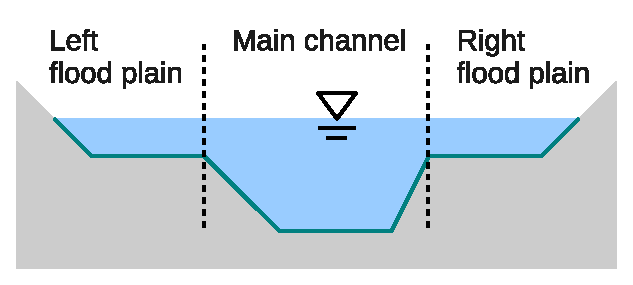
\includegraphics[width=0.55\columnwidth]{\figdir/xs-geometry-simple.eps}
  \caption{A typical river cross-section. \label{fig:xsanalyzer:geometry}}
\end{figure}

The cross-sections's geometry can be represented as a two column table. One column specifies the offset from a fixed point (typically at the left bank) and the other column holds the corresponding elevations. From such a table, the functions $A(D)$ and $R(D)$ can instantly be computed, where $D$ is the maximum flow depth in the cross-section, $A$ is cross-sections the wet area, and $R$ is the hydraulic radius (wet area divided by the wet perimeter).

Using Manning's equation (\eqnref{eqn:xsanalyzer:manning}), the flow rate for steady uniform conditions $Q$ can be calculated for a given flow depth $D$ if the slope $S$ and the roughness parameter $n$ are known. The reverse computation aimed at finding the value of $D$ for a given $Q$ is also possible but requires a numerical solution.

\begin{equation}
  Q(D) = \frac{1}{n} \cdot \sqrt{S} \cdot A(D) \cdot R(D)^{2/3} \label{eqn:xsanalyzer:manning}
\end{equation}

For many real-world cross-sections, the use of a single, unique roughness parameter $n$ is not appropriate. This is often the case for cross-sections with flood plains (\figref{fig:xsanalyzer:geometry}) because the actual surface roughness is horizontally variable. For example, the flood plains may be covered by vegetation while the bed of the main channel is made of sand or concrete. Then, energy losses due to turbulence will be quite different in the channel and the flood plains.

To handle this situation, \software{xsAnalyzer} uses the idea of compound cross-sections \citep[see][]{Cunge1980}. Thus, the cross-section is horizontally sub-divided into separate zones. To each zone, a unique value of $n$ is applied when using \eqnref{eqn:xsanalyzer:manning}. In the case shown in \figref{fig:xsanalyzer:geometry}, for example, the flow rate would be computed in two steps. First, the individual flow rates of the main channel and the two flood plains would be calculated, before the three values are added up in a second step.

It is important to keep in mind that this approach allows for different flow velocities in the zones. In reality, this would lead to additional turbulence and, consequently, result in additional energy losses due to shear at the zones' interface (\figref{fig:xsanalyzer:shear}). Such losses, however, are difficult to estimate and they are \emph{totally neglected} by \software{xsAnalyzer}.

\begin{figure}
  \centering
  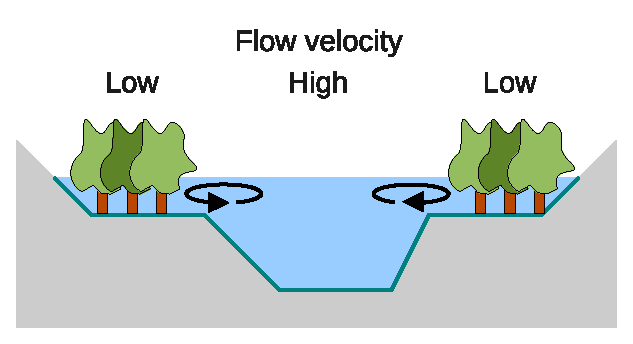
\includegraphics[width=0.55\columnwidth]{\figdir/xs-geometry-shear.eps}
  \caption{Turbulence due to shear at the interface of flow zones. \label{fig:xsanalyzer:shear}}
\end{figure}

If \software{xsAnalyzer} detects a water surface elevation which is higher than the cross-section's elevation at the first and/or last offset, it assumes a vertical wall at the respective offset. The output file (\secref{sec:xsanalyzer:output}) contains a field to detect those critical situations.

%%%%%%%%%%%%%%%%%%%%%%%%%%%%%%%%%%%%%%%%%%%%%%%%%%%%%%%%%%%%%%%%%%%%%%%%%%%%%%%%
%%%%%%%%%%%%%%%%%%%%%%%%%%%%%%%%%%%%%%%%%%%%%%%%%%%%%%%%%%%%%%%%%%%%%%%%%%%%%%%%
%%%%%%%%%%%%%%%%%%%%%%%%%%%%%%%%%%%%%%%%%%%%%%%%%%%%%%%%%%%%%%%%%%%%%%%%%%%%%%%%
\section{Arguments and invocation of \software{xsAnalyzer}} \label{sec:xsanalyzer:args}

\software{xsAnalyzer} is an application written in C++. It expects all input to be supplied as command line arguments. All arguments must be supplied in a keyword-values style as in the following example call:

\begin{lstlisting}[style=shell]
xsAnalyzer file_xsection="geometry.txt"
  file_flows="flowsOfInterest.txt"
  file_out="output.txt"
  read_3d=false
  read_roughness=false
  default_roughness=30
  slope=0.000485
  plain_length=1000.
  max_nreserv_kalmil=100
  print_only_routing=false
\end{lstlisting}

The meaning of the various keywords is as follows:

\begin{columndef}
  \item[file\_xsection] (\textit{string}) Input file with cross-section geometry data. See \secref{sec:xsanalyzer:input:geometry} for details.
  \item[file\_flows] (\textit{string}) Input file listing flow rates of interest. See \secref{sec:xsanalyzer:input:flows} for details.
  \item[file\_out] (\textit{string}) File name/path for output.
  \item[read\_3d] (\textit{logical}) Must be \false{} if the geometry data are given as a table of corresponding offsets and elevations. Must be \true{} if the geometry data are available as 3-dimensional coordinates.
  \item[read\_roughness] (\textit{logical}) Must be \true{} if the table with geometry data contains an additional column with roughness values. Note that the roughness must be specified as Strickler's $Kst$ parameter which is the inverse of Manning's $n$ ($Kst = 1/n$). If \false{}, a unique roughness value is assumed (see next argument).
  \item[default\_roughness] (\textit{numeric}) The unique value of the roughness parameter to be used if no values are specified in the geometry file. Note that the roughness must be specified as Strickler's $Kst$ parameter which is the inverse of Manning's $n$ ($Kst = 1/n$).
  \item[slope] (\textit{numeric}) Slope of the river bed as a dimensionless number (\ie{} meters elevation per meters distance).
  \item[plain\_length] (\textit{numeric}) Length of the reach as a horizontal distance. For typical values of the slope, this is almost identical to the actual length of the reach. 
  \item[max\_nreserv\_kalmil] (\textit{integer}) A parameter to control the output. It specifies the maximum number of conceptual linear reservoirs for the Kalinin-Miljukov routing method.
  \item[print\_only\_routing] (\textit{logical}) A switch to optionally reduce the amount of output information.
\end{columndef}

After successful execution, the return code of \software{xsAnalyzer} is zero. If the program terminates due to an error, a non-zero code is returned and traceback info is sent to standard output.

%%%%%%%%%%%%%%%%%%%%%%%%%%%%%%%%%%%%%%%%%%%%%%%%%%%%%%%%%%%%%%%%%%%%%%%%%%%%%%%%
%%%%%%%%%%%%%%%%%%%%%%%%%%%%%%%%%%%%%%%%%%%%%%%%%%%%%%%%%%%%%%%%%%%%%%%%%%%%%%%%
%%%%%%%%%%%%%%%%%%%%%%%%%%%%%%%%%%%%%%%%%%%%%%%%%%%%%%%%%%%%%%%%%%%%%%%%%%%%%%%%
\section{Input} \label{sec:xsanalyzer:input}

\subsection{Geometry data} \label{sec:xsanalyzer:input:geometry}
The file holding the geometry data must be in tabular format with columns separated by the TAB character (ASCII character code 9). Lines with an initial \verb!#! character are treated as comment lines. A header line with column names is mandatory. See the examples below for the expected column names.

\figsref{fig:xsanalyzer:input:geometry-2D-withoutRoughness} -- \ref{fig:xsanalyzer:input:geometry-3D-withRoughness} illustrate the four different possible file formats for geometry data. If the data are given in 2-dimensional format, the offsets must be in increasing order.

Note that, of roughness information is present, the value for a particuar offset applies to the part of the cross-section between this offset and the following offset. Thus, the roughness information of the very last record is effectively ignored (but a value must be present).

\begin{figure}
\begin{lstlisting}[style=txt]
  offset   z
  -100     20
  0        20
  5        15
  25       15
  30       20
  100      20
\end{lstlisting}
  \caption{Example of geometry file in 2D format without roughness information. \label{fig:xsanalyzer:input:geometry-2D-withoutRoughness}}
\end{figure}

\begin{figure}
\begin{lstlisting}[style=txt]
  offset   z     Kst
  -100     20    20
  0        20    30
  5        15    30
  25       15    30
  30       20    20
  100      20    20
\end{lstlisting}
  \caption{Example of geometry file in 2D format with specified roughness. \label{fig:xsanalyzer:input:geometry-2D-withRoughness}}
\end{figure}

\begin{figure}
\begin{lstlisting}[style=txt]
  x      y   z
  -100   0   20
  0      0   20
  5      0   15
  25     0   15
  30     0   20
  100    0   20
\end{lstlisting}
  \caption{Example of geometry file in 3D format without roughness information. \label{fig:xsanalyzer:input:geometry-3D-withoutRoughness}}
\end{figure}

\begin{figure}
\begin{lstlisting}[style=txt]
  x      y   z     Kst
  -100   0   20    20
  0      0   20    30
  5      0   15    30
  25     0   15    30
  30     0   20    20
  100    0   20    20
\end{lstlisting}
  \caption{Example of geometry file in 3D format with specified roughness. \label{fig:xsanalyzer:input:geometry-3D-withRoughness}}
\end{figure}

\subsection{Flow values of interest} \label{sec:xsanalyzer:input:flows}
The flow data are read from a plain text file like the one in \figref{fig:xsanalyzer:input:flows}. This is effectively a single-column table. A header must not be present. The user is free to specify a list of flow values with arbitrary increments but the data must be in increasing order.

\begin{figure}
\begin{lstlisting}[style=txt]
0.1
1
2
5
10
50
100
\end{lstlisting}
  \caption{Example of file with flow data for use with \software{xsAnalyzer}. \label{fig:xsanalyzer:input:flows}}
\end{figure}

\subsection{Units} \label{sec:xsanalyzer:input:units}
Note that the units of all input data need to be consistent. If, for example, the offsets are given in meters, the elevation data must be provided in units of meters too. At the same time, flow rates must be given in units of \cbm{} per second.

%%%%%%%%%%%%%%%%%%%%%%%%%%%%%%%%%%%%%%%%%%%%%%%%%%%%%%%%%%%%%%%%%%%%%%%%%%%%%%%%
%%%%%%%%%%%%%%%%%%%%%%%%%%%%%%%%%%%%%%%%%%%%%%%%%%%%%%%%%%%%%%%%%%%%%%%%%%%%%%%%
%%%%%%%%%%%%%%%%%%%%%%%%%%%%%%%%%%%%%%%%%%%%%%%%%%%%%%%%%%%%%%%%%%%%%%%%%%%%%%%%
\section{Output} \label{sec:xsanalyzer:output}
The current version of \software{xsAnalyzer} generates a single output file containing a summary of the properties of the cross-section / reach. An example is shown in \figref{fig:xsanalyzer:output}.

\begin{sidewaysfigure*}
{\small
\begin{lstlisting}[style=txt]
# Cross-section property table          
#   X-section data file:    in/montalban/geometry_constRough.txt          
#   Flow data file:         in/montalban/flowsOfInterest.txt          
#   Used reach length:      1000          
#   Used slope:             0.000485          
#   Used roughness: 30 (Global default)          
flow stage overtop wet_area top_width wet_perimeter volume_total dvdq_total nsub volume_sub dvdq_sub
0.5  19.74 0       1.71     5.6       5.79          1707.2       2231.8     3    569.1      743.9
1    19.92 0       2.82     6.94      7.19          2823.1       2111.8     2    1411.6     1055.9
2    20.16 0       4.69     8.74      9.07          4694.9       1915.7     1    4694.9     1915.7
5    20.64 0       10.84    18.02     18.57         10836.9      1932.4     1    10836.9    1932.4
10   21.02 0       19.54    27.94     28.67         19541.2      1553.4     1    19541.2    1553.4
20   21.41 0       31.33    32.13     32.98         31326.8      1175.3     1    31326.8    1175.3
30   21.75 0       43.05    38.84     39.73         43046.2      1310.8     1    43046.2    1310.8
50   22.33 0       74.82    72.4      73.55         74819.0      1302.6     1    74819.0    1302.6
75   22.64 0       98.45    78.1      79.51         98446.4      849.8      1    98446.4    849.8
100  22.88 0       117.31   78.32     80.04         117309.9     727.7      1    117309.9   727.7
\end{lstlisting}
}
  \caption{Example of an output file produced by \software{xsAnalyzer}. \label{fig:xsanalyzer:output}}
\end{sidewaysfigure*}

The meaning of the columns is as follows:
\begin{columndef}
  \item[flow] Flow rates of interest as specified in the input file.
  \item[stage] Water surface elevations corresponding to the flow rates of interest.
  \item[overtop] Either 0 or 1. A value of 1 means that the water surface elevation is higher than the cross-sections elevation at the first and/or last offset. In that case, a vertical wall was assumed as a boundary.
  \item[wet\_area] Wet cross-section area.
  \item[top\_width] Cross-section top width.
  \item[wet\_perimeter] Wetted perimeter.
  \item[volume\_total] Total storage volume of the reach.
  \item[dvdq\_total] Estimated derivative of the storage volume with respect to the flow rate.
  \item[nsub] Suggested number of linear reservoirs (= length of cascade) for Kalinin-Miljukov routing.
  \item[volume\_sub] Storage volume in the individual reservoirs for Kalinin-Miljukov routing.
  \item[dvdq\_sub] Estimated derivative of the storage volume with respect to the flow rate for the individual reservoirs for Kalinin-Miljukov routing. 
\end{columndef}
